\chapter{Casimir effect}\label{cha:casimir-effect}

General introduction and comparison with retarded van der Waals forces

\begin{equation}\label{eq:3:casimir-pp-F-conducting}
  F_\mathrm{Casimir} = - \frac{\hbar c \pi^2}{240 L^4} A
\end{equation}

\begin{equation}\label{eq:3:casimir-pp-E-conducting}
  V_\mathrm{Casimir} = \frac{\hbar c \pi^2}{720 L^3} A
\end{equation}


Lifshitz:
\begin{equation} \label{eq:3:casimir-pp-F-DD-lifshitz}
  F_\mathrm{DD} = \frac{\hbar c \pi^2}{240 L^4} \left( \frac{\varepsilon_r - 1}{\varepsilon_r + 1} \right)^2 \varphi(\varepsilon_r)
\end{equation}
\begin{equation}\label{eq:3:casimir-pp-F-DM-lifshitz}
  F_\mathrm{DM} = \frac{\hbar c \pi^2}{240 L^4} \frac{\varepsilon_r - 1}{\varepsilon_r + 1} \varphi(\varepsilon_r)
\end{equation}

The numeric function $\varphi$ is shown in \cref{fig:casimir-numeric}.


\begin{figure}[!htbp]
  \centering
  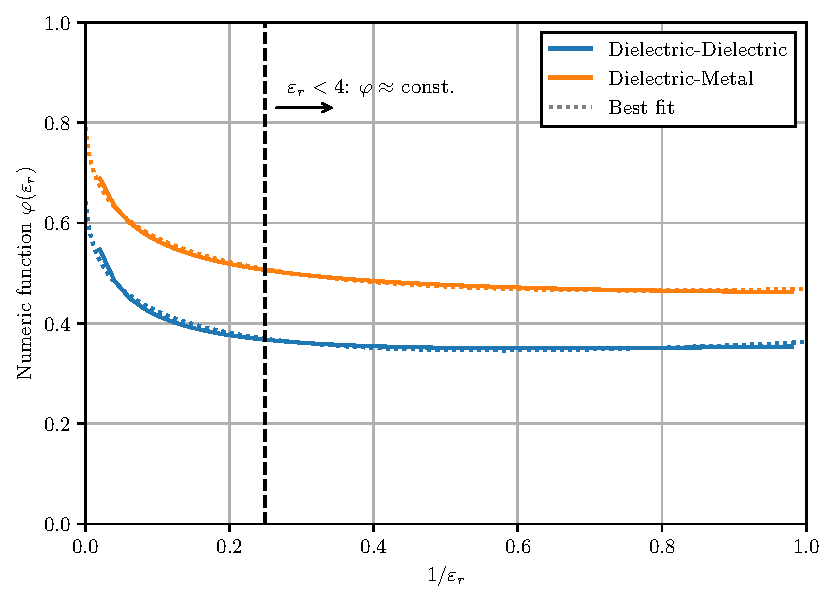
\includegraphics[width=\textwidth]{./../figures/casimir-numeric.pdf}
  \caption{Numeric casimir interaction $\varphi(\epsilon_r)$ between \textbf{(blue)} two dielectric plates and \textbf{(orange)} a dielectric and a conductor.}
  \label{fig:casimir-numeric}
\end{figure}


\section{Proximity force approximation}
The Casimir-Polder force cannot be calculated easily for different shapes. There even exists no analytic expression for the simple (and for this thesis relevant) plate-sphere geometry for all ratios $L/R$ and plate-sphere separations.
For a general shape, even the sign of the force, i.e. whether it is attractive or repulsive, is often unknown.
Fortunately, approximation methods exist and in particular the \emph{proximity-force-approximation (PFA)} can be calculated very easily \cite{Hartmann_2018,Emig_2007a,Bulgac_2006}.
The PFA is only valid for small separations ($L/R \approx 1$) between the considered smooth bodies.
The idea of this approximation is to divide the surfaces of the two bodies into infinitesimal small parallel plates with area $\dd A$ and summing over the forces $\dd F$ (or the Casimir-energy $\dd E$) between them (see \cref{fig:3:PFA}):
\begin{equation}\label{eq:3:pfa}
  E_\mathrm{PFA} = \iint_A \dd A \, \frac{E_\mathrm{plate-plate}}{A}
\end{equation}
where for the casimir energy per unit area $E_\mathrm{plate-plate}/A$ either eq. \eqref{eq:3:casimir-pp-E-conducting} or any of the Lifshitz equations \eqref{eq:3:casimir-pp-F-DD-lifshitz}, \eqref{eq:3:casimir-pp-F-DM-lifshitz} can be chosen.
\begin{figure}[!htbp]
  \centering
  \def\svgwidth{0.55\textwidth}
  \input{./../figures/proximity-force-approximation.pdf_tex}
  \caption{In the proximity force approximation the sphere is divided into infinitesimal plane areas $\dd A$ which all exert a force $\dd F$ according to eq. \eqref{eq:3:casimir-pp-F-conducting}. All the contributions are added up together.}
  \label{fig:3:PFA}
\end{figure}
For the following calculations, it is important to distinguish between the distance between the plates center and the spheres center $L$ (like used before) and the edge-to-edge distance $\mathscr{L} = L - R$.

The problem with this approximation is, that it is ambiguous, what surface the area element $\dd A$ represents. For the plate-sphere geometry, the element can be either chosen tangential to the sphere or parallel to the plate (or in theory any other fictitious surface somewhere in between) \cite{Bulgac_2006}.
For the plate-sphere geometry, in the limit of the validity of the PFA $\mathscr{L} \ll R$ both methods yield the same result.
For the following calculations, I choose $\dd A$ parallel to the plate and the area can be parameterized with $r\in [0, R]$ and $\varphi \in [0, 2\pi]$ resulting in a distance $z$ between the infinitesimal area elements $z(r) = \mathscr{L} + R - \sqrt{R^2 - r^2}$ \footnote{Taking $\dd A$ tangential to the sphere, it can be parameterized with $\theta \in [0, \pi/2]$ and $\varphi \in [0, 2\pi]$ resulting in $z(\theta) = \mathscr{L} + R - R\cos\theta$. The PFA eq. \eqref{eq:3:pfa} yields with $\dd A = R^2\sin\theta\dd\theta\dd\varphi$ the result $\propto \frac{\pi R^2(R + 2\mathscr{L})}{\mathscr{L}^2(R+\mathscr{L})^2}$ which in the limit of $\mathscr{L} \ll R$ results in the same expression as eq. \eqref{eq:3:PFA-sphere-plate}.}. The PFA eq. \eqref{eq:3:pfa} then yields for a dielectric sphere against a perfectly conducting plate
\begin{align}
  E_\mathrm{plate-sphere} &= -\frac{\hbar c \pi^2}{720} \left(\frac{\varepsilon_r - 1}{\varepsilon_r + 1}\right) \varphi(\varepsilon_r) \int_0^R \dd r \int_0^{2\pi} r\dd \varphi \frac{1}{z(r)^3} \\
  &= -\frac{\hbar c \pi^3}{360} \left(\frac{\varepsilon_r - 1}{\varepsilon_r + 1}\right) \varphi(\varepsilon_r) \frac{R^2}{2\mathscr{L}^2(R + \mathscr{L})} \\
  &\approx -\frac{\hbar c \pi^3}{720} \left(\frac{\varepsilon_r - 1}{\varepsilon_r + 1}\right) \varphi(\varepsilon_r) \frac{R}{\mathscr{L}^2} \label{eq:3:PFA-sphere-plate}
\end{align}



\section{Imperfect plate and spheres}

Python numerical approach, gaussian modes (vibration modes of a spherical plane), perlin noise



\section{Casimir forces between a conducting plate and a dielectric sphere}
\subsection{Polarizability of a dielectric sphere}
The polarizability $\alpha$ is defined via
\begin{equation}
  \vec{E_\infty} \alpha = \vec{p},
\end{equation}
where $\vec{p}$ is the induced dipole moment and $\vec{E_\infty}$ is the external electric field that induces the dipole moment. For a linear and uniform dielectric, it is given as $\vec{p} = \mathcal{V} \varepsilon_0 (\varepsilon_r - 1) \vec{E_\mathrm{in}}$ \cite[p. 220-226]{Griffiths_2018}. Here, $\mathcal{V}$ is the volume of the object and $\vec{E_\mathrm{in}}$ is the electric field inside the dielectric.
The electrostatic boundary conditions for the problem are given by
\begin{equation}
  V_\mathrm{in} \big|_{r=R} = V_\mathrm{out} \big|_{r=R} 
  \quad \text{and} \quad 
  \varepsilon_r\varepsilon_0\pdv{V_\mathrm{in}}{r}\bigg|_{r=R} = \varepsilon_0\pdv{V_\mathrm{out}}{r} \bigg|_{r=R}
\end{equation}
and the electric potential outside of the sphere at $r\rightarrow\infty$ should be equal to the external dipole-inducing field $V_\mathrm{out} |_{r\rightarrow\infty} = -\vec{E_\infty} \cdot \vec{r} = -E_\infty r\cos\theta$.
The electric potential inside and outside the sphere can be calculated using the spherical decomposition of the general electric potential $V \propto 1/\abs{\vec{r} - \vec{r'}}$ into Legendre Polynomials $P_l$ \cite[p. 188-190]{Griffiths_2018}:
\begin{align}
  V_\mathrm{in}(r, \theta) &= -E_\infty r\cos\theta + \sum_{l=0}^{\infty} A_l r^l P_l(\cos\theta), \\
  V_\mathrm{out}(r, \theta) &= -E_\infty r \cos\theta + \sum_{l=0}^{\infty} \frac{B_l}{r^{l+1}} P_l(\cos\theta).
\end{align}
Applying both boundary conditions, it follows that \cite[p. 249-251]{Griffiths_2018}
\begin{equation}
  \begin{cases}
    A_l = B_l = 0 & \text{for } l \neq 1, \\
  A_1 = -\frac{3}{\varepsilon_r + 2}E_\infty, \quad B_1 = \frac{\varepsilon_r-1}{\varepsilon_r + 2}R^3E_\infty
  \end{cases}
\end{equation}
and the resulting  homogenous electric field $\vec{E_\mathrm{in}} = -\vec{\nabla} V_\mathrm{in}$ inside the sphere is given as
\begin{equation}
  \vec{E_\mathrm{in}} = \frac{3}{\varepsilon_r + 2} \vec{E_\infty} .
\end{equation}
The field is shown on the right in \cref{fig:dielectric-sphere-field}.The polarizability $\alpha$ of the sphere can be now be determined to
\begin{equation}
  \alpha_\mathrm{sphere} = 4\pi \varepsilon_0 R^3 \left(\frac{\varepsilon_r - 1}{\varepsilon_r + 2}\right).
\end{equation}

% \begin{figure}[!htbp]
%   \centering
%   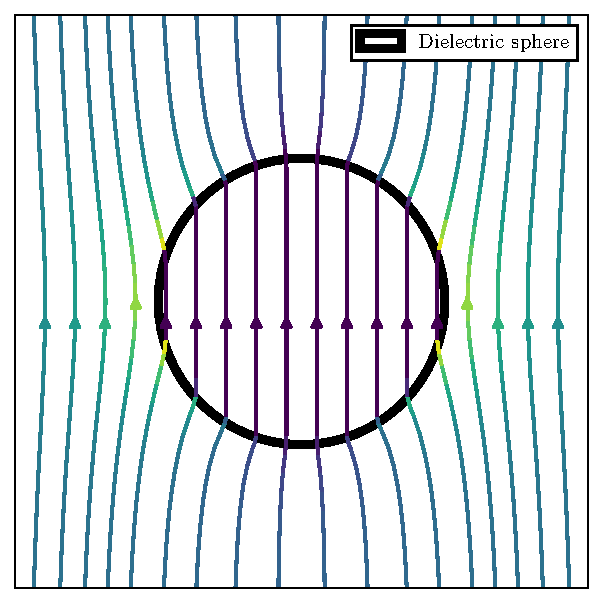
\includegraphics[width=0.8\textwidth]{./../figures/field-dielectric-sphere.pdf}
%   \label{fig:field-dielectric-sphere}
%   \caption{Electric field lines through an dielectric sphere}
% \end{figure}

\begin{figure}[!htbp]
  \centering
  \begin{subfigure}[b]{0.48\textwidth}
      \centering
      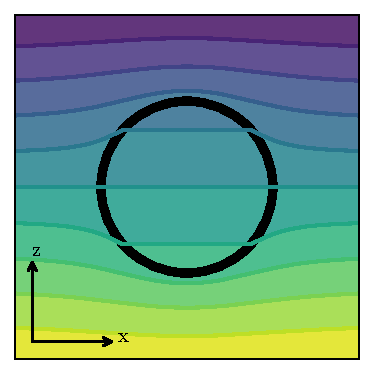
\includegraphics[width=\textwidth]{./../figures/potential-dielectric-sphere-small.pdf}
  \end{subfigure}
  \hfill
  \begin{subfigure}[b]{0.48\textwidth}
      \centering
      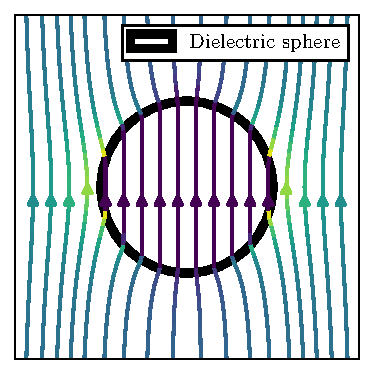
\includegraphics[width=\textwidth]{./../figures/field-dielectric-sphere-small.pdf}
  \end{subfigure}
  \caption{\textbf{left:} Electric potential $V$ of a dielectric sphere in a external electric field $\vec{E_\infty} \parallel \vec{e_z}$. \textbf{right:} The corresponding electric field lines inside and outside the dielectric sphere.}
  \label{fig:dielectric-sphere-field}
\end{figure}